\section{Finance Simulation}
\label{sec:diag}
Nike, Salih\\

The finance simulation is connected to almost all other simulations, as costs and profits are ruling an enterprise's daily work. The main financial key figure is the company net worth. A company's net worth is the difference between assets and liabilities\footnote{https://www.investopedia.com/terms/n/networth.asp}. In a successful company, this value should be positive and increase continuously. This is shown in a balance sheet that is updated annually. The picture below shows an example of the balance sheet in CapitalismX which is updated monthly for the calculations in the backend. On the assets side there are non-current assets, which include buildings, machinery, vehicle fleets and investments, and current assets, which include components, products, bank and cash. On the liabilities side, the equity capital and the liabilities are shown including loans and payables. However, in CapitalismX the company net worth as well as all other financial key figures are calculated in a simplified manner, due to the high complexity in the real world.\\

\begin{figure}
	\centering
	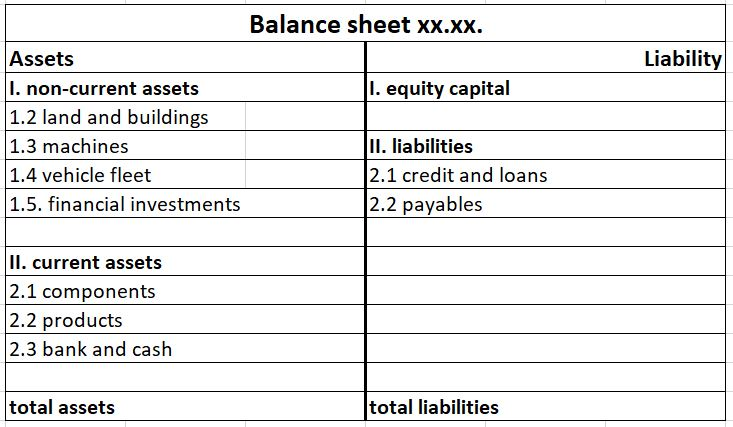
\includegraphics[width=12cm]{images/balance sheet.JPG}
	\caption{Example Balance Sheet in CapitalismX}
\end{figure}


% Nike, weißt du wieso über dem Graphen function graph.JPG steht?
\begin{figure}
	\centering
	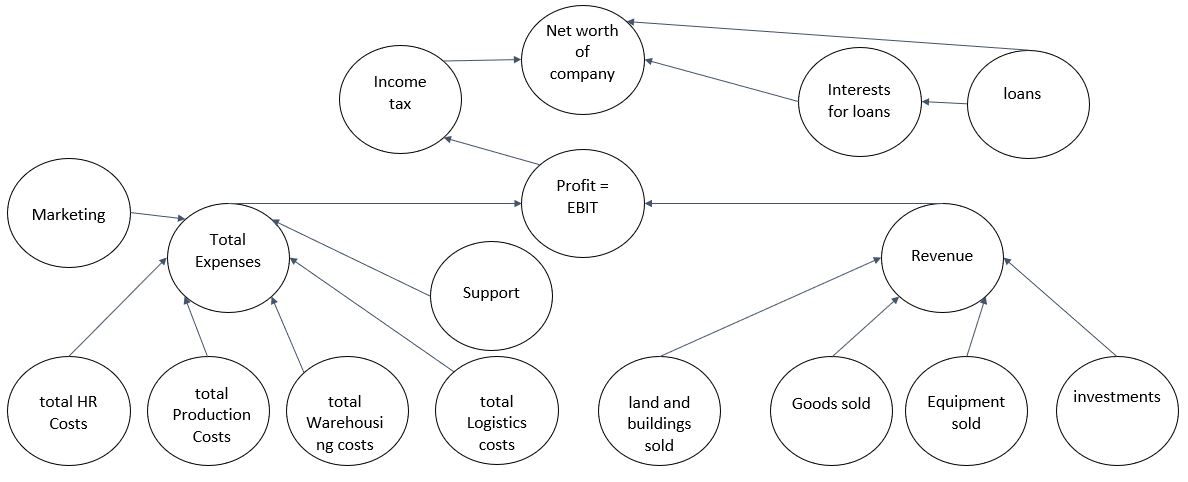
\includegraphics[width=12cm]{images/cost function graph.JPG}
	\caption{Finance Simulation Overview}
\end{figure}

The company’s net worth is calculated from the EBIT, that the player has obtained through his or her actions during the game. Added to the EBIT there are the loans a player might have borrowed from the bank, the interest that the player has to expend in order to amortize the loan, and the income tax the player has to pay for all earnings. \\
$$net worth= (EBIT+loan\ amount+(loan\ interests/365))* taxPercentage$$
[insert formula]
Net worth = EBIT + loan amount + (loan interests /360) if day == 01, then Net worth = (EBIT + loan amount + (loan interests / 360) ) * taxPercentage.

Net worth is an ad hoc calculated key figure, which means that periodically occurring costs, such as interests for loans, that are due on a monthly basis are not included until the beginning of the next month. 

 to 20\% is
 
 
In CapitalismX the income tax is levied on a monthly basis and can be compared to the income tax paid by a large corporation in the United States of America according to the IAS 12 \textit{Income Taxes} paragraph from the IFRS\footnote{https://www.ifrs.org/-/media/feature/meetings/2018/october/iasb/ap12c-ias12.pdf}, although of course realistically the income tax is levied annually. In order to provide the player a more structured overview about the company’s financial situation, we decided to provide the player with a monthly income tax, that is subtracted from the net worth. Hence, at the beginning of a month the net worth decreases by the amount calculated with the tax e.g. net worth = current net worth * (1-tax percentage). However, by hiring powerful lobbyists, the income tax percentage can be decreased down to a total value of 10 \%, which is explained in chapter [CHAPTER REFERENCE].\\

As already mentioned, borrowings and interest rates are added to EBIT. Similar to the calculation of the income tax, the loan repayments and interest rates are recorded on the first day of each month. As a result, net worth decreases by these amounts at the beginning of each month.\\
The bank simulation ensures that the player has an additional opportunity to raise capital in case of bottlenecks or for investments. Three types of credit are offered to the player in case of a request. 
The short-term loan requires a repayment within one and twelve months. The interest rate varies between 6\% and 18\%. The medium-term loan is payable within 1-5 years, while the interest rate is between 3\% and 6\%. A long-term loan has a term of more than 10 years (maximum 15 years?) with an interest rate between 1\% and 3\% \footnote{https://www.statista.com/statistics/258174/long-term-interest-rates-worldwide}. The bank's credit offers are randomized in the defined intervals to make the game more interesting for the player. The three types of credit are provided as amortization loans. Thus, the player has a fixed interest rate and a fixed monthly amortization. This reduces the repayment amount over time \footnote{\footnote{https://www.investopedia.com/terms/a/amortized\_loan.asp}}.
However, the raising of capital from the bank is restricted.
The requested loan must not be larger than 30 percent of the company value, which is for reasons of simplification the current company net worth. If this is fulfilled, the player receives three offers. In the event of a negative check by the bank, the player receives an adjusted offer corresponding to the company value. The new loan amount offered is not greater than 30\% of the company value. See the attached activity chart. 

\begin{figure}
	\centering
	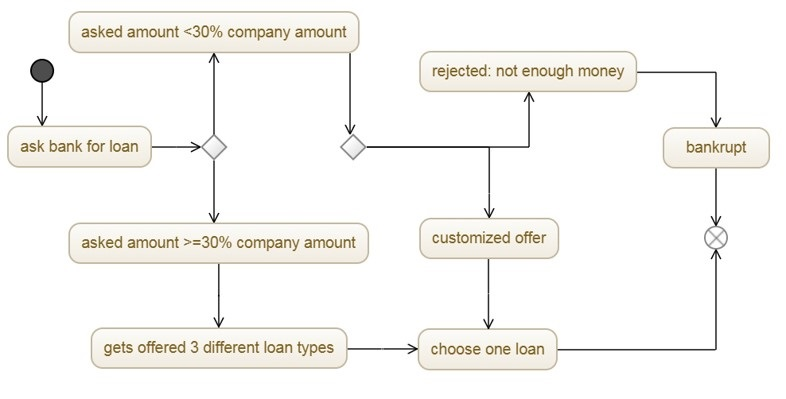
\includegraphics[width=12cm]{images/banking_activity_diagram.jpg}
	\caption{Activity Diagram Banking Simulation}
	\label{jpg:banking}
\end{figure}

The following variables and formulas are defined for the calculation of the repayment, but also for the observation of the bank restrictions.\\

\begin{itemize}
    \item variables:
    \item Principal of Loan = S; retirement= a; term= t; interest rate= i; principal balance per year= S\textsubscript{n}; Rate= r. 
    \item formulas:
 $$a={\dfrac{S}{t}}$$
 $$S_n=S-(a*t)$$
 $$Interest\ rate\ per\ year: i_n=S_t*i $$
 $$Rate\ per\ year: r_t=a+i_t$$
$$Rate\ per\ month:r_m= {\dfrac{r_t}{12}} $$
    
\end{itemize}


The next level under the company net worth is the EBIT, which are the earnings before interest and tax, a commonly used key financial indicator in company's financial statements \footnote{https://www.investopedia.com/terms/e/ebit.asp} [REFERENCE]. Again, the calculation of the EBIT is simplified for the business simulation game at hand. All revenues are added to the EBIT and the total expenses are subtracted. Revenues are the sum of all incoming cash flows, which are:
\begin{itemize}
    \item Goods sold, displayed by the total sales of products, which can be derived by multiplying a product’s price, which is set by the user with the amount of units sold.
    \begin{equation}
        Sales: S(P) = \sum price\index{Product} * units sold
    \end{equation}
    \item Equipment sold. The player has the possibility to sell used machinery or vehicles, that he or she do not need anymore. The calculation for the residual value can be found in chapter [CHAPTER Reference].
    \item Land and buildings sold, which are calculated similar to the equipment sold and described in chapter [CHAPTER Reference].
    \item Investments, which are either positive or negative incomes from the investment area in the financial dashboard.
\end{itemize}

FUNCTIONS for revenues in this part - SALIH
On the other side, there are the total expenses, which are the costs and expenditures that occur across all other simulations, such as:
\begin{itemize}
    \item Total Salaries from the HR simulation, which is the sum of all salaries. The calculation of these costs can be found in chapter [CHAPTER Reference].
    \item Warehousing costs, which occur when producing more products than the market currently demands. Also, the components which are not manufactured into products yet generate warehousing costs, as they need to be stored somewhere. The calculation of these costs can be found in chapter [CHAPTER Reference]. 
    \item Logistic costs, which occur when selling or retailing products. The calculation of these costs can be found in chapter [CHAPTER Reference].
    \item Production costs, which occur when manufacturing components to products. The calculation of these costs can be found in chapter [CHAPTER Reference].
    \item Marketing costs, which occur when starting marketing activities like marketing campaigns, market research or press releases. The calculation of these costs can be found in chapter [CHAPTER Reference].
    \item support costs, which occur [clarify].. The calculation of these costs can be found in chapter [CHAPTER Reference].
\end{itemize}

This seen, the EBIT can be calculated as follows: [formula]. - NIKE

Describe UI – what is behind the Finance dashboard? E.g. cashflow – all values mentioned above on a quarterly basis, net worth on a daily basis, etc. - SALIH

Financing from within the business is the internal financing, while financing from organizations outside the company is called external financing. Equity financing occurs, when raising money in exchange for a share of ownership in the business whereas borrowing money, that must be repaid over a period of time, is the debt financing. 
In CapX the player has 3 financing options at his disposal. Due to the high complexity financing options such as leasing, factoring, increase of deposits or provisions were not conceptualized. 
The simplest and most common financing in CapX is the sale of products whose profits can be used for new investments. The linear depreciation of machines, trucks and buildings has the advantage that one thing can be converted into CapCoins at the remaining value at the click of a mouse \footnote{https://www.modu-learn.de/verstehen/finanzen/finanzierungsarten/}.
In the event that internal financing is no longer feasible, it is possible to borrow money from the bank. These three financing options are explained in more detail below.

– SALIH

Describe how implemented in prototype: net worth of company equals profit, taxes are not considered - profit equals ebit, so interests and taxes are substracted to get net worth - [should be done, after final implementation]